\section{Results: single-friction sweeps}
\label{sec:results-singles}

This section reports the three single-friction parameter sweeps. Each cell uses 250 sessions of the unified C++ simulator described in Section~\ref{sec:methodology}; reported numbers are means of converged session-level $\Delta$ with cross-session standard deviation in parentheses. All runs converged --- not a single session failed the four-consecutive-episode strategy-stability test within the 1{,}000-episode cap.

\subsection{Friction 1: observation latency}
\label{sec:results-latency}

Table~\ref{tab:latency-results} reports $\Delta$ across the latency grid \(L\in\{0,1,2,3,5,10,20\}\). At \(L=0\) the simulator reproduces the baseline ($\Delta = 0.843$, SD $= 0.114$), confirming the per-agent state implementation reduces correctly to the shared-state baseline. From \(L=0\) to \(L=1\), $\Delta$ collapses from $0.843$ to $0.280$, a sixty-seven-percent reduction from a single period of observation delay. From \(L=1\) onward, $\Delta$ decays further but more slowly, settling near a floor of approximately $0.16$ for \(L\geq 5\). Figure~\ref{fig:latency} plots the curve.

\begin{table}[H]
\centering
\caption{Effect of observation latency on collusion (250 sessions per cell).}
\label{tab:latency-results}
\begin{tabular}{rcc}
\toprule
$L$ (periods) & $\Delta$ & SD \\
\midrule
0  & 0.843 & 0.114 \\
1  & 0.280 & 0.146 \\
2  & 0.215 & 0.110 \\
3  & 0.193 & 0.088 \\
5  & 0.174 & 0.072 \\
10 & 0.158 & 0.054 \\
20 & 0.155 & 0.052 \\
\bottomrule
\end{tabular}
\end{table}

\begin{figure}[H]
\centering
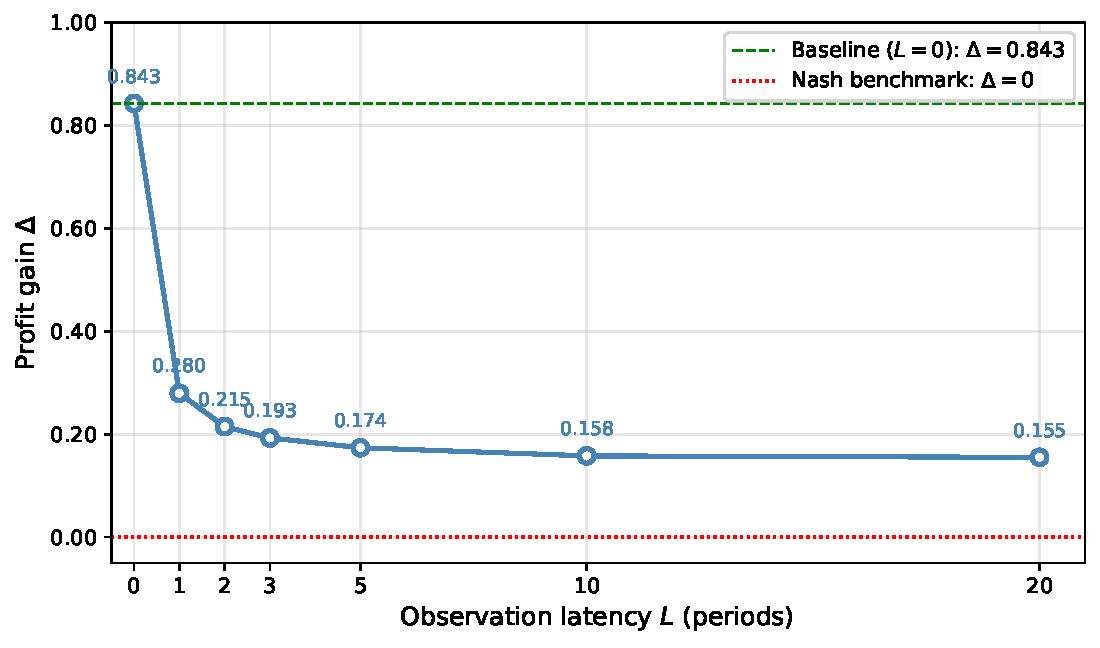
\includegraphics[width=0.78\linewidth]{figures/fig_latency.pdf}
\caption{$\Delta$ as a function of observation latency $L$. The cliff at $L=1$ accounts for nearly the entire effect; further latency adds little.}
\label{fig:latency}
\end{figure}

\paragraph{Interpretation.}
Two features of this curve are worth highlighting. First, the size of the drop at $L=1$ is striking: a single period of delay erases two-thirds of the collusion. The mechanism is that the Calvano baseline relies on the rival's last-period price both as a coordination device and as the input to any retaliation rule. A one-period delay simultaneously breaks both functions. Second, $\Delta$ does not reach Nash even at $L=20$, when an agent is essentially blind for twenty periods. The residual collusion at $\Delta\approx 0.16$ must rest on coordination mechanisms that do \emph{not} require timely monitoring --- most plausibly, agents converge on a stable mutual-high-price focal point that requires no real-time enforcement. This residual is destroyed in Section~\ref{sec:results-noise} when the friction acts on the state \emph{value} rather than on its arrival time.

\subsection{Friction 2: noisy monitoring}
\label{sec:results-noise}

Table~\ref{tab:noise-results} reports $\Delta$ across the noise grid \(\sigma\in\{0, 0.5, 1, 2, 3, 5, 10\}\). At \(\sigma=0\) the result matches the baseline to five decimal places, the bit-for-bit sanity check described in Section~\ref{sec:methodology-noise}. From there $\Delta$ declines smoothly and roughly monotonically: $0.670$ at $\sigma=0.5$, $0.493$ at $\sigma=1$, $0.242$ at $\sigma=2$, falling to essentially Nash ($\Delta=0.013$) by $\sigma=5$. At $\sigma=10$ --- where the noise standard deviation exceeds the entire 15-point price grid and observation is effectively uniform random --- $\Delta=-0.003$, indistinguishable from the Nash benchmark.

\begin{table}[H]
\centering
\caption{Effect of noisy monitoring on collusion (250 sessions per cell).}
\label{tab:noise-results}
\begin{tabular}{rcc}
\toprule
$\sigma$ & $\Delta$ & SD \\
\midrule
0.0  & $\phantom{-}0.843$ & 0.114 \\
0.5  & $\phantom{-}0.670$ & 0.226 \\
1.0  & $\phantom{-}0.493$ & 0.290 \\
2.0  & $\phantom{-}0.242$ & 0.262 \\
3.0  & $\phantom{-}0.143$ & 0.218 \\
5.0  & $\phantom{-}0.013$ & 0.064 \\
10.0 & $-0.003$           & 0.073 \\
\bottomrule
\end{tabular}
\end{table}

\begin{figure}[H]
\centering
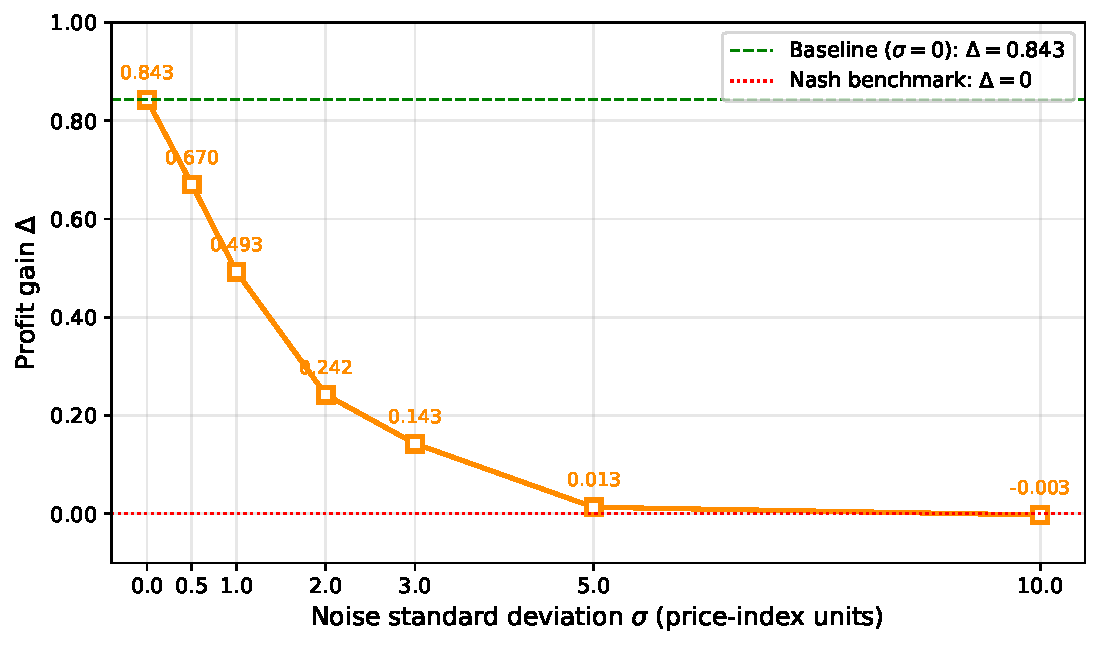
\includegraphics[width=0.78\linewidth]{figures/fig_noise.pdf}
\caption{$\Delta$ as a function of noise standard deviation $\sigma$. Smooth monotone decline; no residual collusion floor.}
\label{fig:noise}
\end{figure}

\paragraph{Interpretation.}
The shape of the noise curve differs from the latency curve in two respects. There is no cliff: the decline from $\Delta=0.843$ to $\Delta\approx 0$ unfolds smoothly across the range $\sigma\in[0,5]$. And there is no residual collusion floor: $\Delta$ at high $\sigma$ converges to the Nash benchmark, not to the $\approx 0.16$ floor seen under heavy latency. The mechanism story is that noise corrupts the \emph{value} of the rival-side state, not its time of arrival. At high $\sigma$ the agent's perceived state is near-independent of the rival's actual price, which means no policy conditioned on that state can encode coordination of any kind, focal or otherwise. Latency leaves the focal-point mechanism intact (the state is correct, just stale); noise destroys it.

The contrast already suggests that the two frictions act through different channels and therefore could compound, the question taken up in Section~\ref{sec:results-factorial}.

\subsection{Friction 3: asynchronous actions}
\label{sec:results-async}

Table~\ref{tab:async-results} reports $\Delta$ across the lock-in grid \(T\in\{0,1,2,5,10,20\}\). At $T=0$ the simulator reproduces the baseline. At $T=1$ --- pure Maskin--Tirole strict alternation --- $\Delta$ drops to $0.378$. From $T=2$ onward the curve plateaus around $\Delta\approx 0.41$, with no further systematic movement up to $T=20$.

\begin{table}[H]
\centering
\caption{Effect of asynchronous actions on collusion (250 sessions per cell).}
\label{tab:async-results}
\begin{tabular}{rcc}
\toprule
$T$ (lock-in length) & $\Delta$ & SD \\
\midrule
0  & 0.843 & 0.114 \\
1  & 0.378 & 0.108 \\
2  & 0.418 & 0.095 \\
5  & 0.424 & 0.116 \\
10 & 0.411 & 0.108 \\
20 & 0.403 & 0.119 \\
\bottomrule
\end{tabular}
\end{table}

\begin{figure}[H]
\centering
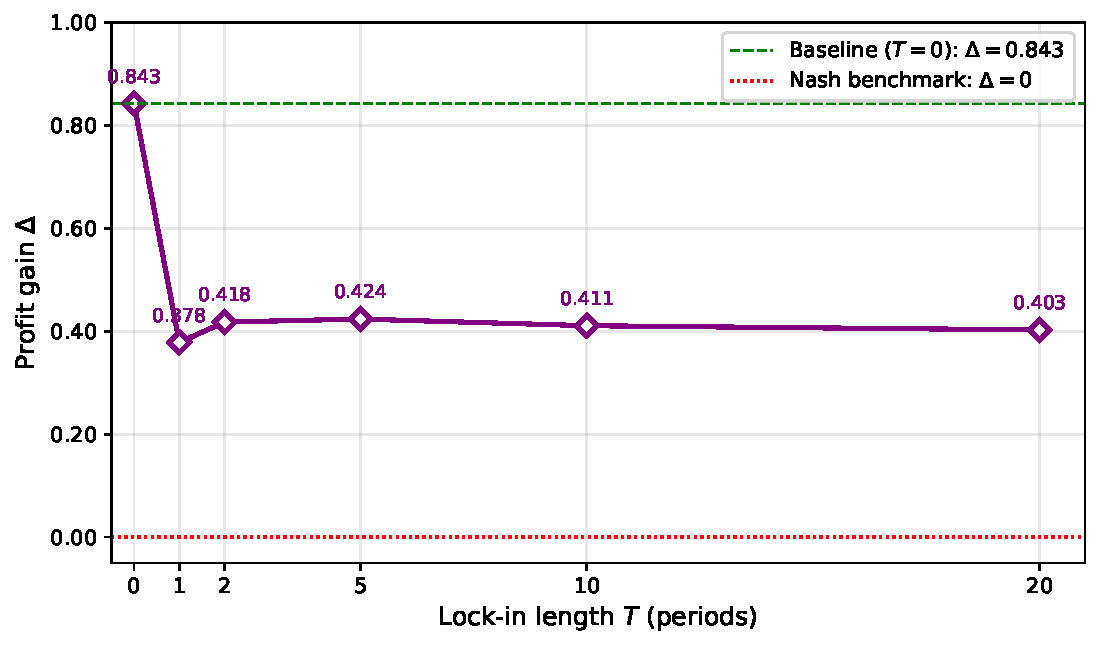
\includegraphics[width=0.78\linewidth]{figures/fig_async.pdf}
\caption{$\Delta$ as a function of asynchrony lock-in length $T$. Step from baseline at $T=0$ to a plateau around $\Delta\approx 0.41$ for $T\geq 1$.}
\label{fig:async}
\end{figure}

\paragraph{Interpretation.}
This curve was the most surprising of the three. The pre-experiment hypothesis, motivated by Maskin--Tirole reaction-function reasoning and \citet{klein2021}'s sequential-pricing results, was that strict alternation should preserve or even enhance collusion: the moving agent faces a known, committed rival price and ought to be able to rationalise a cooperative best-response. The Q-learners do not behave that way at this parameter regime. Mandatory alternation cuts $\Delta$ in roughly half, from $0.843$ to $0.378$ at $T=1$. The plateau at $\Delta\approx 0.41$ for $T\geq 2$ shows that the effect is structural --- it depends on \emph{whether} prices are simultaneous or staggered, not much on \emph{how staggered} they are.

A possible mechanism: under strict alternation, each agent's relevant state-decision pair is restricted to half the periods (only those in which it moves). With $\varepsilon$-greedy exploration and a fixed 5{,}000-iteration episode length, this halves the effective state-visitation rate during learning, and the algorithm has correspondingly more difficulty discovering the high-price equilibria of the baseline. This is a learning-side rather than a strategic-side explanation, distinct from the analytic Maskin--Tirole prediction. Distinguishing the two would require off-path deviation analysis (does the asynchronous equilibrium support punishment? does it survive the genuine-vs-spurious test of \citet{calvano2023}?), which is left to future work.

\subsection{Three shapes side by side}
\label{sec:results-three-comparison}

Figure~\ref{fig:three-friction} places the three single-friction sweeps on a shared $\Delta$ axis. The qualitative differences are visible at a glance.

\begin{figure}[H]
\centering
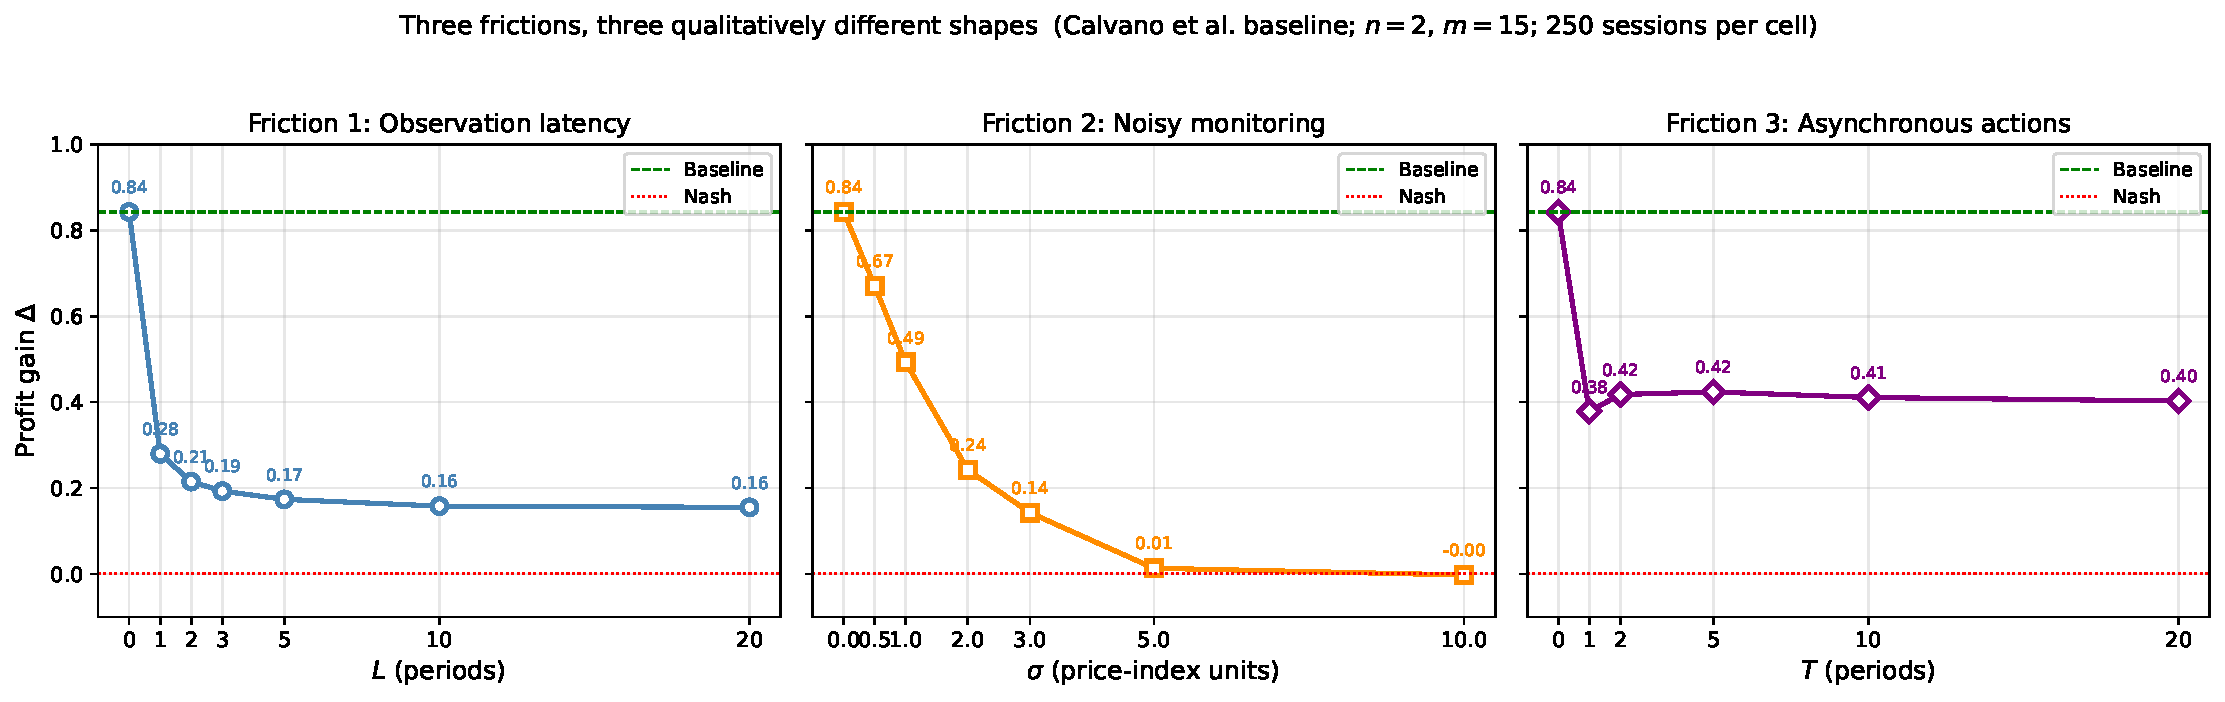
\includegraphics[width=0.99\linewidth]{figures/fig_three_friction_comparison.pdf}
\caption{Three frictions, three qualitatively different shapes. Latency: cliff at $L=1$ then floor at $\Delta\approx 0.16$. Noise: smooth monotone decline to Nash. Asynchrony: step from baseline at $T=0$ to plateau at $\Delta\approx 0.41$.}
\label{fig:three-friction}
\end{figure}

The three shapes correspond to three distinct mechanisms by which information or timing structure can interfere with learned collusion. \emph{Latency} delays signals; \emph{noise} corrupts them; \emph{asynchrony} restructures the game. Each leaves the others intact, which makes them natural candidates for a factorial test.
